\documentclass[11pt]{article}
\usepackage{etex}
\usepackage{amssymb,amsmath,fancyhdr,multicol}

\usepackage{hyperref}

\usepackage[metapost]{mfpic}

%\pgfplotsset{compat=1.9}
%\usepackage{amsmath}
\usepackage[pdftex]{graphicx}
%\usepackage{mystylefortest}
%\usepackage{multicol}
\usepackage{pst-plot}
\usepackage{pgfplots}

\usepackage{tikz}
\usepackage{tkz-2d}
\usepackage{tkz-base}
\usetikzlibrary{calc}

\usepackage[inline]{enumitem}

\textheight 25cm% 25.5cm
\textwidth 18cm \topmargin -2.5cm
\parindent 0pt
\oddsidemargin -1cm \columnsep 18pt 
\renewcommand{\headrulewidth}{0pt}
\pagestyle{fancy} \lhead{}\chead{}\rhead{}
\lfoot{}\cfoot{}\rfoot{}
%\newcommand{\ds}{\displaystyle}

\usepackage{tabularx}
\renewcommand{\tabularxcolumn}[1]{>{\centering\arraybackslash}m{#1}}

\usepackage{array}
\newcolumntype{?}{!{\vrule width 1pt}}

\usepackage[linewidth=1pt]{mdframed}

%\prec 
\pgfplotsset{compat=1.9} %%May have to change to 1.11 at work

\pgfplotsset{soldot/.style={color=blue,only marks,mark=*}} \pgfplotsset{holdot/.style={color=blue,fill=white,only marks,mark=*}}
\pgfplotsset{
  grid style = {
    dash pattern = on 0.05mm off 1mm,
    line cap = round,
    black,
    line width = 0.5pt
  }
}

\newcommand{\vasymptote}[2][]{
    \draw [densely dashed,thick, #1] ({rel axis cs:0,0} -| {axis cs:#2,0}) -- ({rel axis cs:0,1} -| {axis cs:#2,0});
}

\opengraphsfile{TrigFunctionQuestions}

\begin{document}

\centerline{\textbf{Trigonometric Functions Questions}}

\vspace{.5in}

%\textbf{Name:}\hrulefill\

%\vspace{.25in}

%\makebox[\textwidth]{Name:\enspace\hrulefill}
%\vspace{1pt}

%\begin{questions}


%\addpoints
%\qformat{Question \thequestion\dotfill
 %        {(\pointsofquestion{\arabic{question}} \points)}}
        
\begin{enumerate} 



\item  Find the amplitude, period, and phase shift of the function $\displaystyle y=4\sin\left (\frac{1}{2}x-\frac{\pi}{6}\right )$. Sketch the graph.

\item The graph of a complete period of a cosine curve is shown below.

\begin{tikzpicture}
\begin{axis}[
%minor tick num=3,
xmax=2.2,
ymax=2.2,
ymin=-2.2,
axis y line=center,
axis x line=middle,
xlabel=$x$,ylabel=$y$,
xtick={0.5,1,...,2},
xticklabels={%
$\frac{\pi}{4}$,
$\frac{\pi}{2}$}
]

\addplot[smooth,blue,mark=none,
domain=0:2,samples=40]
{2*cos(3.14*\x r)};
\end{axis}
\end{tikzpicture}
\begin{enumerate}
\item Find the amplitude, period and phase shift.
\item Write an equation that represents the curve in the form
$\displaystyle y = a \cos k(x - b)$.
\end{enumerate}
\item Part of the graph of  a cosine curve $f(x)$ is shown below.

\begin{center}
\twoptoff
\begin{tikzpicture}[yscale=1.5, xscale=1.5]
\tkzInit[xmin=-5,xmax=4.01,ymin=-2,ymax=2.15]
\tkzY[gradsize=\scriptstyle]
\tkzX[pos={below right=1pt,}]
\tkzGrid[color=orange]
\draw[color=black,samples at={-5,-4.96,...,4.01}] plot (\x,{sin(3.14/3*(\x +1) r )})%
;
\tkzLegend[color=white!30,lw=1pt](5,2)%
{triangle*/1ex/white/\textbf{$f(x)$}}
\end{tikzpicture}
\twopton
\end{center}
\begin{enumerate}
\item Find the amplitude, period and phase shift.
\item Write an equation that represents the curve in the form
$\displaystyle y = a \cos k(x - b)$.
\end{enumerate}

\item  A trigonometric function is given by $\displaystyle y=2\sin\left (\frac{2}{3}x-\frac{2\pi}{9}\right )$.  Find the amplitude, period, and phase shift of the function. Sketch the graph.

\item Part of the graph of a trigonometric function is shown below.



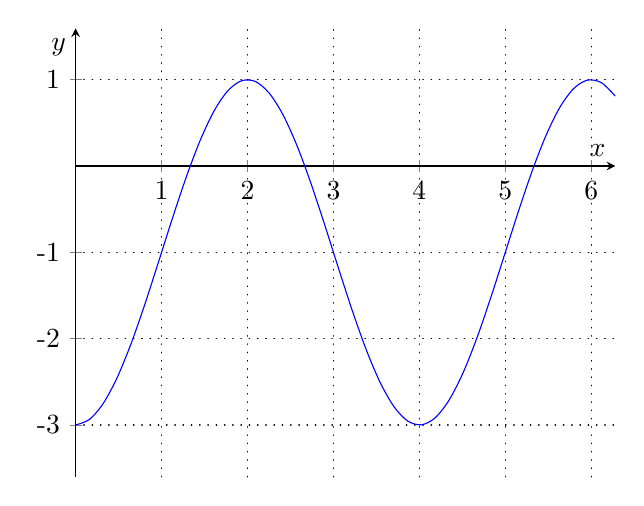
\begin{tikzpicture}
\begin{axis}[
	%minor tick num=3,
axis y line=center,
	axis x line=middle,
	%enlarge x limits=0.15,
        enlarge y limits=0.15,
	every axis y label/.style={at={(current axis.above origin)},anchor=north east},
	xlabel=$x$,ylabel=$y$,xtick={0,1,2,3,4,5,6}, xticklabels={0,1,2,3,4,5,6},ytick={-3,-2,-1,0,1},yticklabels={-3,-2,-1,0,1},grid=both
	]
	\addplot[smooth,blue,mark=none,
		 domain=0:6.28,samples=40] 
		{-1-2*cos(deg(x*pi/2))};
\end{axis}
\end{tikzpicture}

Write an equation that represents the graph, in the form of $\displaystyle y=A\cos K(x-B)+C$ or $\displaystyle y=A\sin K(x-B)+C$. Show your work step-by-step, and clearly explain how you find $A,B,C,K$.

\item Describe a sequence of function transformations that would transform the graph of $f(x)=\sin(x)$ into the graph of $\displaystyle g(x)=2\sin(4x)+6$.

\item A ferris wheel has a diameter of 160 meters and makes one revolution  every 30 minutes. It is constructed so that the lowest part of the wheel reaches ground level, enabling passengers to simply walk on to, and off of, the ride. Find a function $\displaystyle H(x)=A\sin(K(x-B))+C$ which models the height $H$ of the passenger above the ground in meters $x$ minutes after they board the wheel at ground level.

\item In the past few days I have noticed that the temperature in my office fluctuates according to the formula $\displaystyle T(x)=22\sin\left(\frac{\pi}{12}(x-4)\right )+63$, where $x$ is the number of hours since  8 am and $T$ is in degrees Fahrenheit.
\begin{enumerate}
\item What is the highest temperature in my office? 

\item At what time of the day is the temperature the highest? 

\item At what time(s) of the day is the temperature equal to $74^0$F?

\item At what time(s) of the day is the temperature equal to $52^0$F?

\end{enumerate}

\item The number of hours of daylight in a city situate at  latitude $41^0$ North varies between a minimum of 9 hours on December 21st of daylight on December 21st, and a maximum of 15 hours on June 21st. %http://astro.unl.edu/classaction/animations/coordsmotion/daylighthoursexplorer.html
Let $f(x)$ be the number of hours
of daylight  on a day that is $x$ months after December 21st, 2013. 
\begin{enumerate} 
\item Graph one period of the function. Label the axes, include tick marks and label them. Label the coordinates of all peaks and valleys.
\item Use the graph to estimate the times (between December 21st, 2013 and December 21st, 2014) when there are going to be exactly 13.5 hours of sunlight. Write an equation to find these times and solve it. Give your answers in exact form, not as a decimal.
\item Use the graph to estimate the times (between December 21st, 2013 and December 21st, 2014) when there are going to be exactly 13 hours of sunlight. Write an equation to find these times and solve it. Give your answers in exact form, not as a decimal.
\end{enumerate}



\end{enumerate}
\end{document}